\documentclass[a4paper,10pt,twocolumn]{article}
\usepackage{txfonts}
\usepackage[utf8]{inputenc}
\usepackage[cyr]{aeguill}
\usepackage{algorithmic, algorithm}
\usepackage{graphicx}
\usepackage{url}
\urlstyle{sf}

%opening
\title{Creating transparent, steerable recommendations}
\author{
Fran\c{c}ois Maillet\\
Sun Microsystems Inc.\\
University of Montreal\\
\texttt{mailletf@iro.umontreal.ca}
\and 
Paul Lamere \\
Sun Microsystems Inc.\\
\texttt{paul.lamere@sun.com}
}
\date{September 2008}

\begin{document}

\maketitle

\begin{abstract}

Music recommendation systems are increasingly important in the ever 
    growing world of digital music.  However, most commercial music 
    recommenders rely on collaborative filtering techniques to generate 
    music recommendations. These type of recommendations lack two aspects 
    that are important for recommendation.  First, they lack transparency 
    - they cannot explain why an item was recommended beyond the trivial 
    "Other people who listed to XX also listened to YY". Second, they 
    lack steerability - there is no way for a user to interact with the 
    recommender to steer it to more relevant content.
    
    In this demonstration we show the Sun Labs Music Explaura - a 
    web-based recommender that provides transparent and steerable 
    recommendations. The Music Explaura can offer a detailed explanation 
    about why a particular item was recommended and will allow a user to 
    steer the recommendations based upon attributes of the music.

\end{abstract}

\section{Problems with current recommender systems}

they just don't work! you really want to know why?

\section{The Web Music Explaura}

\subsection{The Aura}

In our system for recommending items, each item is
described by a set of words (tags).  These
descriptive words may come from text mining the
web, social annotations, autotagging based upon
content analysis, expert annotation, etc.

The tags are weighted based upon their descriptive
content. More descriptive words are given more
weight.  Standard weighting functions such as
TF-IDF can be used to apply these weights.  This
set of weighted tags for an item is called an
item's "tag cloud", or in a more poetic way, it's aura.

\subsection{Transparency}

A key component of any recommender is the ability to 
find similar items to an item or a set of items. As we represent items using 
a tag cloud, we determine the similarity of two artists by computing the 
cosine distance between their tag clouds.

As shown in figure \ref{fig:commontags}, this allows us to explain why an item is being recommended 
by displaying the overlap between two tag clouds. 

\begin{figure}[ht]
\begin{center}
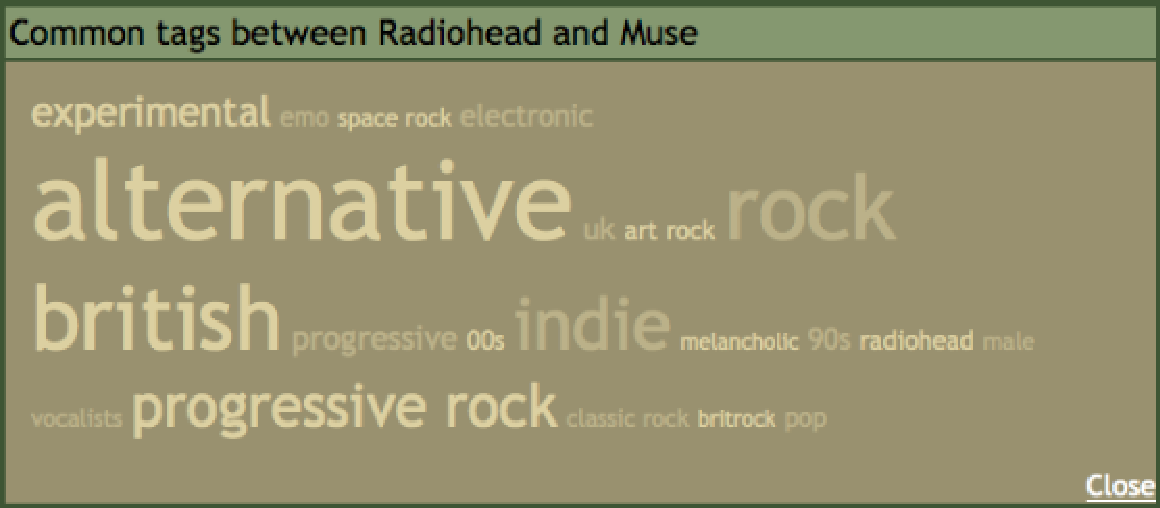
\includegraphics[width=0.9\columnwidth]{radiohead-muse-commontags}
\end{center}
\caption{Common tags between Radiohead and Muse. This tag cloud is displayed as an explanation of why Muse is recommended to a Radiohead listener. The tags in the clouds are weighted by the strength of the overlap between the two clouds.}
\label{fig:commontags}
\end{figure}

\subsection{Steerability}

We can also construct a tag cloud independent of
any particular item and use this as input to the
recommender. This tag cloud describes the
parameters that are important to the user.  The
recommender will use the same 'FindSimilar'
techniques to find items that are similar to the
tag cloud, and return the similar items
(potentially filtered) as recommendations to the
user.  A user can interact with the tag cloud as shown in figure \ref{fig:steerable}.  A
user can dynamically adjust the tag cloud
weights interactively, receiving updated
recommendations in real time after every adjustment. This
allows the user to steer the recommender toward
areas that are of most interest to the user.

\begin{figure*}
\begin{center}
\includegraphics[width=0.95\textwidth]{steerable-withtxt}
\end{center}
\caption{The steerable recommendations interface. Users are able to add tags or artists to the cloud by clicking on them from the right hand panel. Then, they can click and drag them to modify their size. A tag that is shrunk below the size of zero will begin to grow again as a negative tag and act as a filter in the returned recommendations.}
\label{fig:steerable}
\end{figure*}

\end{document}
